\documentclass{beamer}

%\usepackage{beamerthemesplit} // Activate for custom appearance
%\usepackage\{beamercolorthemedove}
%\setbeamertemplate{footline}[textline]{
%
\includegraphics[width=\paperwidth]{figures/datacron_logo.png}}
%}

\usepackage{textpos}
\usepackage{graphicx}
\usepackage{datetime}
\usepackage{tikz}
\usepackage[export]{adjustbox}
\usepackage{natbib}

\usepackage{pgf}
\usepackage{tikz}
\usetikzlibrary{arrows,automata}
%json%
\usepackage{minted}
%sudo apt-get install python-pygments
\usecolortheme{dove}

\def\datacronlogo{%
	\resizebox{!}{2.5ex}{
\includegraphics{figures/datacron_logo.png}%
	}
}
\def\eclogo{
	\resizebox{!}{2.5ex}{
\includegraphics{figures/ec_logo.png}%
	}
}
\def\horizonlogo{%
	\resizebox{!}{2.5ex}{
\includegraphics{figures/horizon_logo.png}%
	}
}

%
\includegraphics[width=\paperwidth]{figures/datacron_logo.png}}

\title{A Distributed Online Learning Approach for Large-scale Pattern Prediction (WP3)}
\author[shortname]{Michael Mock \inst{*} \and Ehab Qadah  \inst{*}}
\institute[shortinst]{\inst{*} Fraunhofer IAIS, Germany \and %
}
\date{\today}

\defbeamertemplate*{footline}{example theme}
{%
	\begin{beamercolorbox}[wd=\paperwidth,ht=2.5ex,dp=1.125ex,%
		leftskip=.3cm,rightskip=.3cm plus1fil]{separation line}
		\usebeamerfont{section in head/foot}%
		\datacronlogo\hfill\insertshorttitle\hfill\dmyydate \today\hfill \thepage \hfill \horizonlogo
	\end{beamercolorbox}
}
\begin{document}
	
	\frame{\titlepage}

	
	\begin{frame}<beamer>
		\frametitle{Outline}
		\tableofcontents
	\end{frame}
	
	
\section{datAcron Architecture}		
\frame
{		
	\frametitle{datAcron Architecture}
	\framesubtitle{}
	
	\begin{center}
		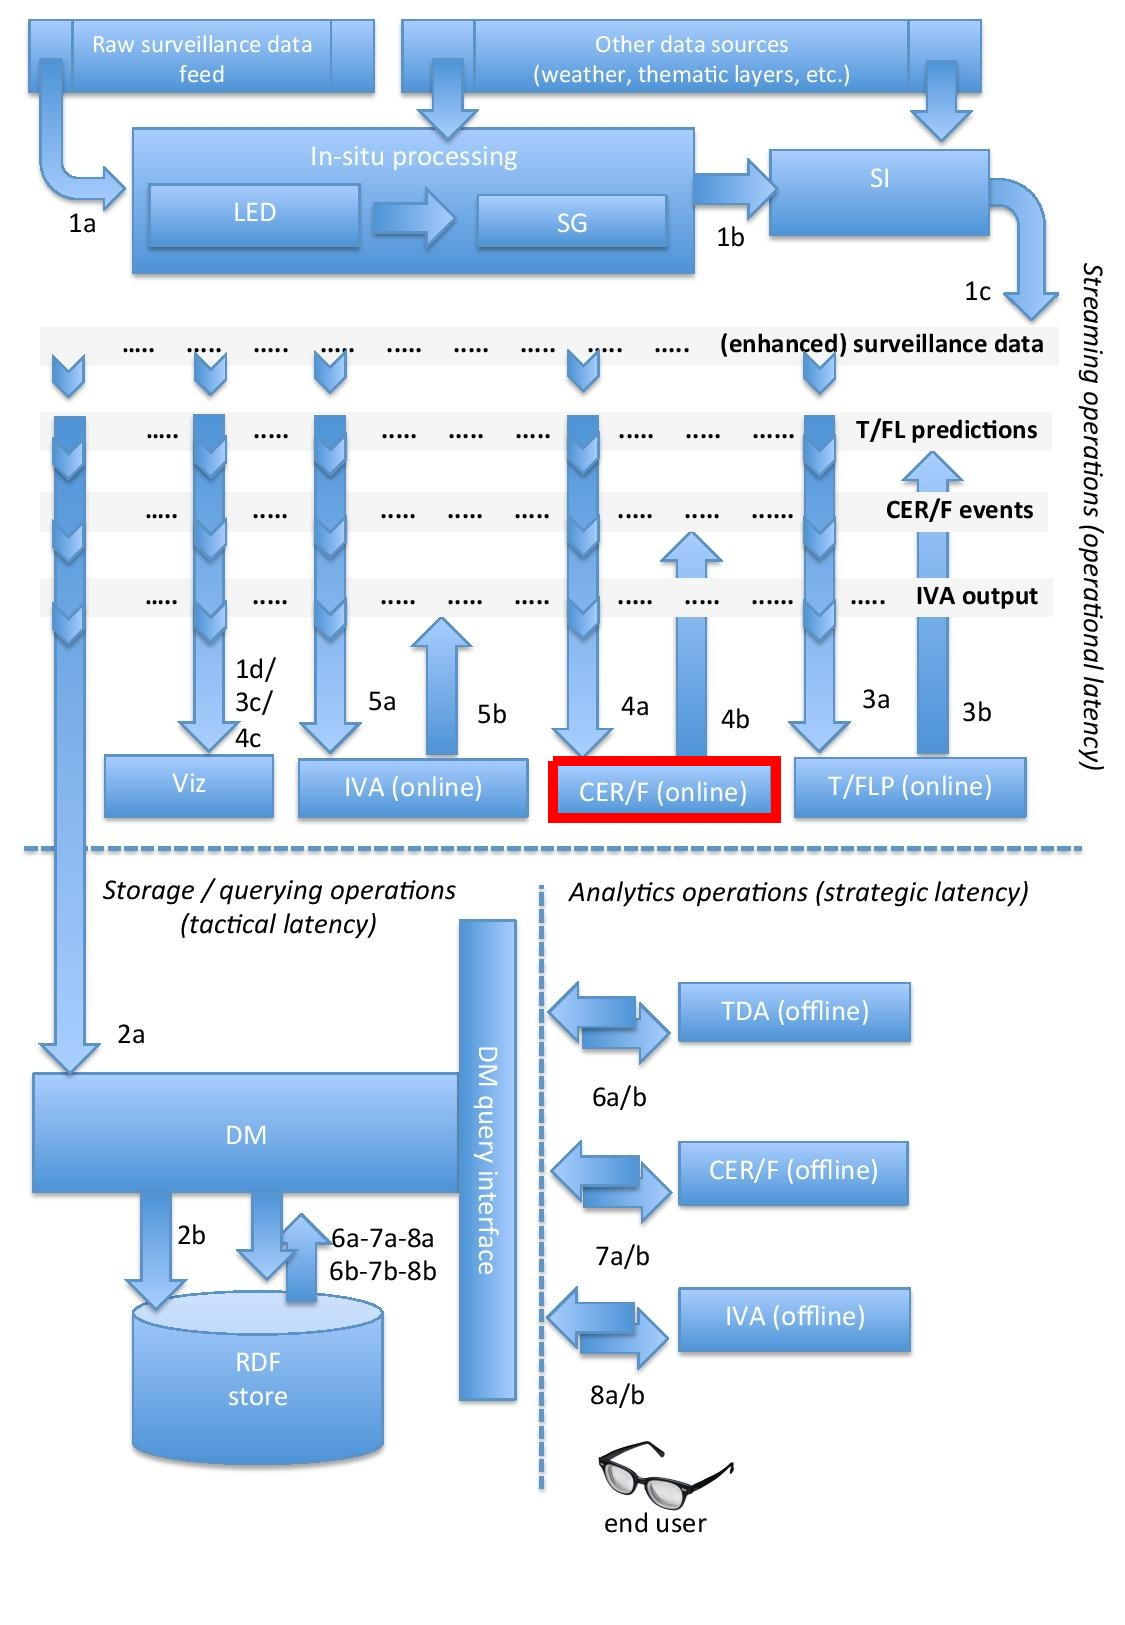
\includegraphics[width=.85\textwidth,height=.75\linewidth]{figures/arch2.jpg}\\
		.
	\end{center}
	
}
\section{Proposed Approach}
\frame
{
	\frametitle{Problem Setting}
	
	\begin{itemize}[]
		\item<1->Given a set of $k$ real-time streams of events $S = \{ s_1,s_2, ..., s_k\}$.
		
		\item<1 -> Each stream $s_i=\langle e_1,e_3...,e_t,...\rangle$  is an evolving time-ordered sequence of events.
		
		\item<1 -> Each event is defined as a tuple of attributes $e_t = (type,\tau,id,a_1,a_2.....,a_n)$ where $type\ \in  \Sigma$ (i.e., event types). 
		\item<1-> A user-defined pattern (i.e., complex event of interest) $P$ expressed as sequence of event types.
		
		%  \item<1->Goal:  provides online prediction about when the event pattern $P$ is expected to be completed each single stream $s_i$ 
		
		\item<1->Goal: the main objective is to predict the pattern $P$ completion with certain probability in the future over each stream $s_i$ given the current time event $e_t$. 
	\end{itemize}
}

\begin{frame}[fragile]
	
	\frametitle{Maritime Surveillance}
	\framesubtitle{}
	\begin{itemize}
		%		\item<only@1> Process  emitted from moving vessels or derived critical points of vessel trajectories as input event streams.
		\item<only@1> Event tuple (i.e., critical points) derived from raw Automatic Identification System (AIS) messages of moving vessels e.g., 
		\begin{minted}{json}
		{
		"timestamp":1443651492000,
		"id":"228133000",
		"annotation":"change_in_heading",
		"latitude":48.117775,
		"longitude":-4.4205885,
		"distance":323.406,
		"heading":264.27
		"speed":18.48,
		}
		\end{minted}
		
		\item<only@1> Example patterns such as 
		$P_1=\mathit{change\_heading} \cdot \mathit{gap\_start} \cdot \mathit{gap\_end} \cdot 
		\mathit{change\_heading}$ or $P_2=\mathit{Sailing}$
	\end{itemize}
\end{frame}


\frame
{
	\frametitle{A Distributed Online Learning Approach for Large-scale Pattern Prediction \footnote{Source Code: https://goo.gl/xwX1Mk}}
	%\framesubtitle{Maritime Surveillance}
	\framesubtitle{Distributed Architecture (Qadah, E., Mock, M., Alevizos, E. \& Fuchs, G. (n.d.))}
	\begin{center}
		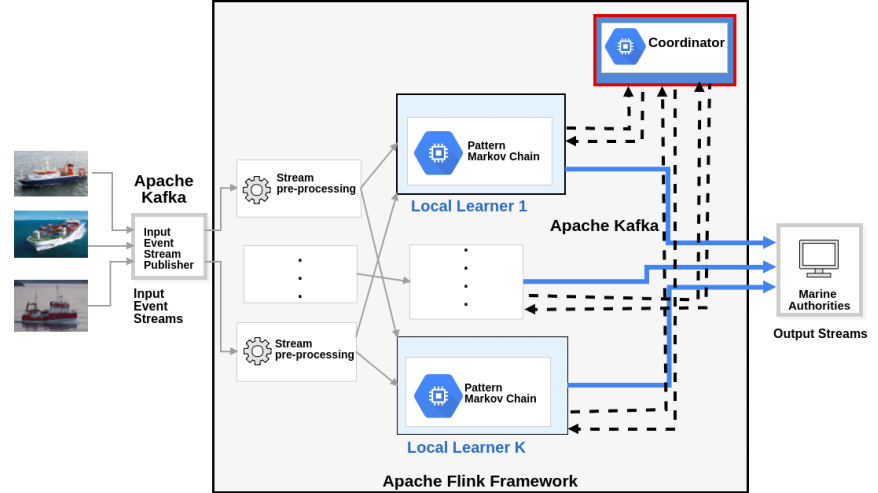
\includegraphics[width=1.05\textwidth,left,height=.58\linewidth]{figures/distributed_architecture_2.png}
.
	\end{center}
}

\subsection{\\ Event Forecasting with Pattern Markov
	Chains\\}
\frame
{
	\frametitle{ Event Forecasting with Pattern Markov
		Chains}
	\framesubtitle{\citep{alevizos2017event}}
	\begin{itemize}[]
		\item<1-> The system consumes a single input stream $s_i$ of events.
		\item<1-> The event stream $s_i$ is assumed to be generated by  $m$-order Markov source.
		\item<1-> The complex event (i.e., pattern) $P$ is defined in the form of regular expressions over a finite set of event types $\Sigma$.
		
		\item<1-> A probabilistic model provides online forecasting reports when the event pattern $P$ is expected to be completed in future. 
		
	\end{itemize}
}


\frame
{
	\frametitle{Event Forecasting with Pattern Markov
		Chains}
	\framesubtitle{How does it work?}
	\begin{itemize}
		\item<only@1> The  deterministic finite automa ($DFA$) is used to construct a Markov chain, which is called a Pattern Markov Chain (PMC).
		
		
		\item<only@1> The states of $DFA$ is directly mapped to states of  transition probability matrix $\boldsymbol{M}$  $\lvert Q \rvert \times \lvert Q \rvert$ of the $PMC$.
		
		\item<only@1> 
		\begin{equation*}
		\label{eq:matrix_example}
		\boldsymbol{M} = 
		\begin{Bmatrix} 
		0 \\ 1 \\ 2 \\ 3 \\4
		\end{Bmatrix}
		\begin{pmatrix} 
		p_{0,0}	    &. 		&. 		& . &  	p_{0,4} \\
		. 		    & .		& .	& .	& . \\
		.		    & .		& .		& .	& . \\
		.			& .		& .		& .	& .\\
		0			& .			& .		& .	&p_{4,4}
		\end{pmatrix}
		\end{equation*}
		
		\item<only@1> The maximum-likelihood estimator is used to compute the transition probabilities (i.e., learning) $p_{i,j}$ of the matrix $\boldsymbol{M}$ 
		\begin{equation}
		\label{eq:pi_estim}
		\hat{p}_{i,j}=\frac{n_{i,j}}{\sum_{k \in Q} n_{i,k}}=\frac{n_{i,j}}{n_{i}}
		\end{equation}. 	
		
	\end{itemize}
}

\subsection{Communication-Efficient Distributed Online Prediction by Dynamic Model Synchronization}
\frame
{
	\frametitle{ Communication-Efficient Distributed Online Prediction by Dynamic Model Synchronization  }
	\framesubtitle{\citep{kamp2014communication}}
	\begin{itemize}[]
		\item<1-> A protocol for distributed online prediction over multiple input data streams in a communication efficient manner.
		\item<1-> It allows to combine local models into a global model
	using a $synchronization$ $ operation$.
		\item<1-> The distributed learners exchange their local model with a central coordinator node periodically after observing a fixed number of data points (i.e., mini-batches) \citep{dekel2012optimal}.
		
		\item<1-> A dynamic synchronization scheme based on monitoring the local models variance from a global reference model ($\|f_i - r\|^2 \leq \bigtriangleup$).
		
		
%		dynamic synchronization scheme within which the learners communicate only if their local models diverge from a global reference point
	\end{itemize}
}


\frame
{
	\frametitle{ Communication-Efficient Distributed Online Prediction by Dynamic Model Synchronization}
	\framesubtitle{}
	\begin{center}
		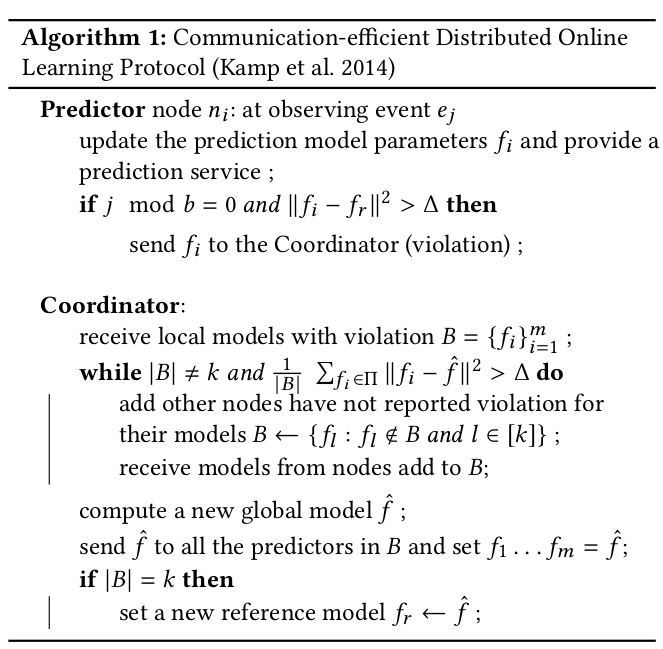
\includegraphics[width=\textwidth,left,height=.8\textheight]{figures/dol.png}\\
		.
	\end{center}
}

\frame
{
	\frametitle{A Distributed Online Learning Approach for Large-scale Pattern Prediction}
		\framesubtitle{Synchronization Operation}
	\begin{itemize}[]

	\item<1->\ We propose a \textit{synchronization operation} for the parameters of the models ($f_i=\boldsymbol{\Pi}_i :i \in[k]$) of the $k$ distributed PMC predictors. The operation is based on distributing the maximum-likelihood estimation for the transition probabilities of the underlying  models described by: 
	\begin{equation*}
	\label{eq:dis_pi_estim}
	\hat{\pi}_{i,j}=\frac{\sum_{k \in K} n_{k,i,j}}{\sum_{k \in K} \sum_{l \in L} n_{k,i,l}}
	\end{equation*}
	
\item<2-> We measure the divergence of local models from the reference model  $\|f_k - f_r\|^2$ by calculating the sum of square difference between the transition probabilities  $\boldsymbol{\Pi}_i$ and  $\boldsymbol{\Pi}_r$:
	\begin{equation*}
	\label{eq:dis_pi_varinace}
	\|f_k - f_r\|^2=\sum_{i,j} (\hat{\pi}_k{i,j} -\hat{\pi}_r{i,j})^2
	\end{equation*}

	
\end{itemize}
}
	\section{EMPIRICAL EVALUATION}
\label{sec:results}
In this section, we evaluate the performance of our system using real-world event streams provided by the datAcron project in the context of maritime domains. The used event streams describe trajectory critical points (i.e., synopses) of moving vessels, which are derived from raw AIS messages as was  described in \cite{synopses1}. In particular, for our evaluation we used a data set of synopses contains $4,684,444$ critical points of $5055$ vessels sailing in the Atlantic Ocean during the period from 1 October 2015 to 31 March 2016. We use it to generate a simulated stream of event tuples  \textit{(id,type,timestamp, longitude, latitude, annotation, speed, heading)},    where $type$ $\in \Sigma$ and $\Sigma=$ $\{$\textit{VerySlow ,Slow, Moving, Sailing, Stopping} $\}$ that is based on the  vessel speed, and $annotation$ is an attribute to encode the trajectory movement events such as speed change, slow motion, and gap in reporting. In our experiments, we monitor a pattern $\mathcal{P}=Sailing$ that detects when the vessel under way (sailing).


\subsubsection*{Experimental setup} We ran our experiments on single-node standalone Flink cluster deployed on a server (Ubuntu 17.04) with Intel(R) Core(TM) i7-7700 CPU @ 3.60GHz X 8 processors and 32GB RAM. We used Apache Flink v1.3.2 and Apache Kafka v0.10.2.1 for our tests.


\subsubsection*{Evaluation criteria} Our goal is to evaluate our distributed pattern prediction based on enabling the synchronization of PMC models between the predictors against the isolated ones (i.e., without exchanging information), we compare the predictive performance in terms of :
\begin{enumerate*}[label=(\roman*)]
	
\item  average $\mathit{precision = \frac{\#\ of\ correct\ predictions}{\#\ of\ total\ predictions}}$ per predictor node

\item $\mathit{cumulative\ error}$ that presents the aggregated number of all wrong predictions.

\item $\mathit{recall}$ that measures the fraction of actual full matches of the defined pattern does the model predicate at least once in previous prediction report

\end{enumerate*} 
Moreover, we study the communication cost by measuring the $\mathit{cumulative\ communication}$ that captures the number of  synchronization related messages, which is introduced by employing the static or dynamic synchronization schemes of the distributed online learning protocol. In next, we present the experimental results for the for the pattern  $\mathcal{P}=Sailing$ with $m=2$, batch size $b=100$,  variance threshold $\Delta=2$, and PMC prediction threshold $\theta_{fc}=80\%$.

\begin{figure}[]
	
	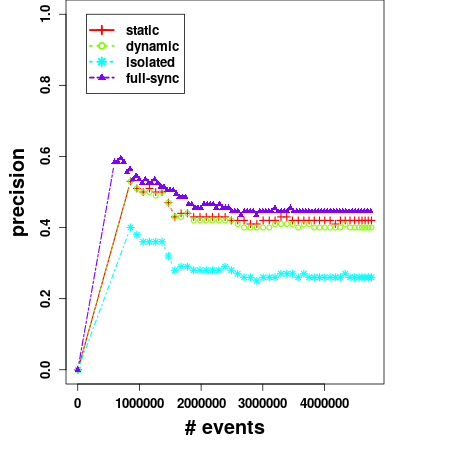
\includegraphics[width=.5\textwidth]{figures/precision.png}
	
	\caption{Precision scores.}
	\label{fig:precsions}
\end{figure}

\subsubsection*{Experimental results} Figure ~\ref{fig:precsions} depicts the precision scores (i.e., average precision of prediction model per vessel)  of all approaches, namely, isolated without synchronization, continuous synchronization, static (periodic), and our proposed approach based on the dynamic synchronization scheme. While Figure ~\ref{fig:error} shows the average cumulative error per predictor.       


\begin{figure}[]
	
	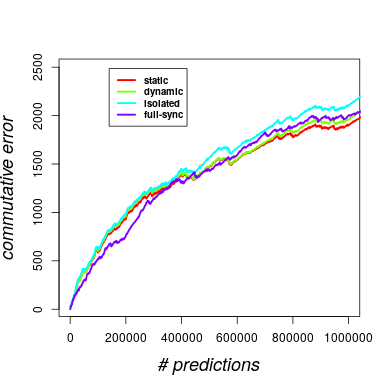
\includegraphics[width=.5\textwidth]{figures/error.png}
	
\caption{Commutative error.}
\label{fig:error}
\end{figure}

\par In Table ~\ref{tab:recall}, we present the statistics of recall results for the different approaches. It can be seen 


\begin{figure}[]
	
	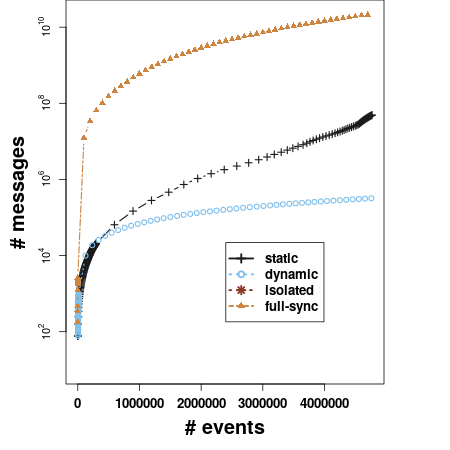
\includegraphics[width=.5\textwidth]{figures/communication.png}
	
	\caption{Commutative communication.}
	\label{fig:comm}
\end{figure}
\begin{table}[]
	\caption{Recall results.}
	\label{tab:recall}
	\begin{tabular}{lll}
		\toprule
		Approach &Mean&Max\\
		\midrule
		isolated & 0.1948  & 0.23 \\
		static & 0.1976  &  0.23 \\
		dynamic & 0.1974  & 0.23 \\
		full-sync & 0.1979  & 0.33 \\
		\bottomrule
	\end{tabular}
\end{table}


Figure ~\ref{fig:comm} provides the accumulated communication required for the three approaches based on the distributed online learning. As expected, larger amount of communication is required for the continuous synchronization comparing to static and dynamic approaches, and it can bee seen with small variance threshold $\Delta=2$ that we can reduce the communication using the dynamic synchronization and comparing the (static) periodic method, and furthermore, still preserving the predictive performance as was shown in Figures ~\ref{fig:precsions} and ~\ref{fig:error}.  


	
	%\begin{frame}
	%\frametitle{Tasks}
	%\begin{columns}
	%\begin{column}{0.5\textwidth}
	%  \begin{itemize}
	%  \item<1->Task 1. 
	%  \end{itemize}
	%\end{column}
	%\begin{column}{0.5\textwidth}  %%<--- here
	%  \begin{itemize}
	%  \item<1-> Task 2. 
	%  \end{itemize}
	%\end{column}
	%\end{columns}
	%\end{frame}
	
	\begin{frame}
		\frametitle{Bibliography}
		\bibliographystyle{agsm} 
		\bibliography{refs}
		
	\end{frame}
\end{document}
